%----------------------------------------------------------------------------------------
%	METODE
%----------------------------------------------------------------------------------------

\section*{METODE PENELITIAN}

Penelitian yang dilakukan terbagi menjadi beberapa tahapan proses. Gambar \ref{fig:tahapan} menunjukan tahapan proses tersebut.

\begin{figure}[h!] % Gunakan \begin{figure*} untuk memasukkan Gambar
	\centering
	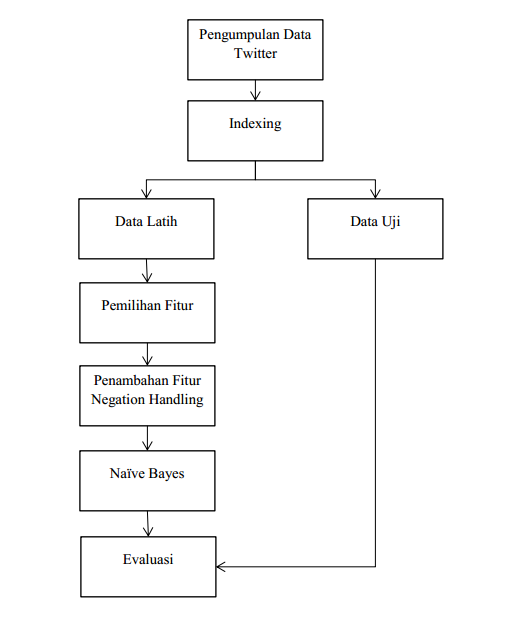
\includegraphics[width=200pt]{langkahkerja.png}
	\caption{Tahapan proses penelitian}
	\label{fig:tahapan}
\end{figure}

\subsection*{Pengumpulan Data}

Penelitian ini menggunakan data twitter bahasa Indonesia. Data yang akan diambil dari twitter adalah data dengan term “Kementrian”, “Menteri”, “Pendidikan”, “Sekolah” dan “Indonesia”. Data dengan term tersebut diambil karena di ranah kementrian sangat membutuhkan opini-opini masyarakat untuk meningkatkan kualitas dari kementrian terkhusus pada ranah Pendidikan. 
Pada tahap akuisisi data tweet, data diperoleh dari tags.hawksey.info. Data yang didapatkan berupa data excel dengan atribut seperti pada Tabel \ref{tab:strukturdatatwitter}.

\begin{table}[hbt]
	\caption{Struktur Data Response Twitter}
	\centering
	\begin{tabular}{llr}
		
		\cmidrule(r){1-2}
		Atribut & Keterangan \\
		\midrule
		id\_str & id dari \textit{post} twitter \\
		from\_user & \textit{username} pemakai twitter \\
		text & \textit{post} twitter \\
		created\_at & tanggal dan waktu \textit{post} dibuat \\
		geo\_coordinates & koordinat tempat \textit{user} \\
		source & tautan profil \textit{user} \\
		profile\_image\_url & gambar profil dari \textit{user} \\
		user\_followers\_count & jumlah \textit{follower user} \\
		user\_friends\_count & jumlah teman \textit{user} \\
		user\_location & lokasi dari \textit{user} \\
		status\_url & link dari \textit{post} twitter \\
		
		\bottomrule
	\end{tabular}
	\label{tab:strukturdatatwitter}
\end{table}

Dari struktur data yang didapatkan dari sistem tersebut, akan diambil atribut "text" sebagai data untuk diolah sentimennya. Data yang diperoleh dari sistem masih berupa data mentah \textit{post user} yang belum ada sentimennya. Untuk memberikan sentimen pada data tersebut yang akan digunakan sebagai data latih dilakukan dengan memberikan opini secara manual dengan bantuan manusia. Penelitian ini menggunakan data sebanyak 6000 data.


\subsection*{Indexing}

\textit{Indexing} merupakan proses persiapan yang dilakukan terhadap dokumen sehingga dokumen siap untuk diproses. Proses \textit{indexing} dibagi menjadi dua proses, yaitu \textit{document indexing} dan \textit{term indexing}. Dari \textit{term indexing} akan dihasilkan koleksi kata yang akan digunakan untuk meningkatkan performansi pencarian pada tahap selanjutnya.  Selain itu, teknik \textit{indexing} ini juga dilakukan agar hasil yang diperoleh lebih baik. Karena kebanyakan tweet hanya berisi tautan dan tidak menunjukkan sentimen tertentu, dan penulisannya ditulis dalam bahasa asing (yang bukan bahasa Inggris)(Parikh dan Movassate, 2014). Tahap-tahap yang dilakukan didalam proses \textit{indexing} meliputi \textit{tokenizing}, pengahapusan \textit{stopwords}, normalisasi kata, \textit{stemming}, pembuatan \textit{document term matrix}.


\subsection*{Tokenizing}
Tokenizing adalah pengambilan kata-kata (term) dari kumpulan dokumen menjadi kumpulan term dan juga membuang beberapa karakter seperti tanda baca. Contoh dari tokenisasi adalah seperti pada tabel \ref{tab:tokenizing}.

\begin{table}[hbt]
	\caption{Tokenizing}
	\centering
	\begin{tabular}{llr}
		\toprule
		Input & \multicolumn{2}{c}{Data Twitter} \\
		\midrule
		Output & Data & Twitter \\
		\bottomrule
	\end{tabular}
	\label{tab:tokenizing}
\end{table}

Proses memotong dokumen atau kata menjadi bagian-bagian yang lebih kecil disebut token. token bisa berupa paragraf, kalimat, frasa kata tunggal sederhana dan konsep. teknik yang digunakan dalam proses tokenisasi adalah segmentasi dan memilah.
Dalam tahap ini dokumen atau data \textit{post} twitter diubah menjadi kumpulan \textit{term} dengan cara menghilangkan \textit{mention}, URL, tanda baca dan angka pada tweet. Semua huruf pada tweet diubah menjadi huruf kecil. Pada penelitian ini tokenisasi dilakukan dengan menggunakan kode dari Nette yang terdapat di https://github.com/nette/tokenizer.


\subsection*{Penghapusan Stopwords}

Stopwords adalah sebuah kata-kata dalam bahasa tertentu yang sangat umum dan memiliki nilai informasi nol. Meyer et.al.(2008). Stopwords didefinisikan sebagai term yang tidak berhubungan (\textit{irrelevant}) dengan dokumen meskipun kata tersebut sering muncul di dalam dokumen. Contoh \textit{stopwords} dalam bahasa  Indonesia : yang, juga, dari, dia, kami, kamu, aku, saya, ini, itu, atau, dll.
Penghapusan stopwords dilakukan untuk menghilangkan kata dalam daftar kata buang (\textit{stopwords}). Kata tersebut merupakan kata yang jika dihapus tidak mengubah makna dari tweet. Daftar \textit{stopwords} didapatkan dari penelitian Tala (2003) sebanyak 759 kata.


\subsection*{Normalisasi Kata}

Menurut Aziz (2013) tahap normalisasi kata dilakukan dengan penggantian kata yang tidak baku menjadi baku, karena kata yang sudah baku akan cenderung lebih kecil ambiguitas dalam pelafalannya dibanding dengan kata yang tidak baku. Misalnya, kata dengan dapat ditulis dengan "dg" dan "dgn".  Untuk itu perlu dilakukan normalisasi kata dengan cara mengganti kata yang tidak baku dengan kata yang sesuai konteknya (Sproat et al. 2001). Sebelumnya sudah dibuat terlebih dahulu sebuah kamus yang tidak baku dengan kata bakunya, agar memudahkan dalam fungsi penggantian dan kemudian menggantinya dengan kata baku yang telah ada di dalam kamus tersebut. Dataset kata tidak baku dan kata baku yang digunakan sebanyak 3719 baris data. 

\subsection*{Stemming}

\textit{Stemming} adalah  proses  konversi term ke bentuk  umumnya. Dokumen dapat pula diekspansi dengan mencarikan  sinonim  bagi \textit{term} tertentu di  dalamnya. Sinonim adalah kata-kata yang mempunyai pengertian serupa tetapi berbeda dari sudut pandang morfologis. Seperti \textit{stemming},  operasi ini bertujuan menemukan suatu kelompok kata terkait.
\textit{Stemming} merupakan salah satu cara yang digunakan untuk meningkatkan performa IR dengan cara mentransformasi kata-kata dalam sebuah dokumen teks ke kata dasarnya (Agusta, 2009). Tahap \textit{stemming} bertujuan untuk mengurangi jumlah kata dan mendapatkan kata dasar yang benar-benar sesuai.Tahap ini menggunakan algoritme Nazief dan Adriani (1996) untuk menghapus berbagai variasi \textit{prefix} (awalan) dan suffix (akhiran). Kamus kata dasar sebanyak 28.526 kata.

\subsection*{Pembuatan Document Term Matrix (DTM)}

Menurut Nadilah (2016) tahap pembuatan \textit{term document matrix} (TDM) dilakukan untuk membuat matriks jumlah kemunculan suatu kata pada dokumen. \textit{Document Term Matrix} (DTM) merupakan cara yang paling umum digunakan untuk merepresentasikan text. DTM dapat diekspor dari korpus dan digunakan sebagai mekanisme \textit{bag-of-words}. Pendekatan ini menghasilkan matrik dengan id dokumen sebagai baris dan \textit{term} sebagai kolom. Elemen matrik merupakan frekuensi.
Sebagai contoh ada dua dokumen dengan id 1 dan 2 mempunyai kata yang sama yaitu “Nama saya budi dan nama ayah saya budi” dan “nama teman saya budi”. Term document matrix yang terbentuk adalah seperti pada Tabel \ref{tab:dtm}.

\begin{table}[hbt]
	\caption{Document Term Matrix}
	\centering
	\begin{adjustbox}{max width=\textwidth}
		\begin{tabular}{*{7}{c}}%%{llr}
			\toprule
			ID & nama & saya & budi & dan & ayah & teman \\
			\midrule
			1 & 2 & 2 & 2 & 1 & 1 & 0 \\
			2 & 1 & 1 & 1 & 0 & 0 & 1 \\
			\bottomrule
		\end{tabular}
	\end{adjustbox}
	\label{tab:dtm}
\end{table}

Pada penelitian ini kolom matriks menunjukkan kata yang ada pada data tweet, sedangkan baris matriks menunjukkan indeks dari dokumen pada kumpulan korpus. Pada penelitian ini satu tweet menandakan satu dokumen.

\subsection*{Pembagian Data}

Data yang dihasilkan setelah proses \textit{indexing} dibagi  menjadi  dua subset data yaitu data latih dan data uji dengan perbandingan 70:30. Sebanyak 70 persen data latih dan 30 persen data uji. Data latih ini akan digunakan untuk tahapan selanjutnya sementara data uji digunakan untuk melakukan pengujian terhadap sistem klasifikasi yang telah dibuat dalam penelitian ini.

\subsection*{Pemilihan Fitur}

Seleksi fitur merupakan proses pemilihan subset dari \textit{term} pada data training. Fitur yang terpilih pada seleksi fitur ini akan digunakan dalam klasifikasi teks. Tujuan dari seleksi fitur adalah membuat data latih yang digunakan \textit{clasifier} lebih efisien dengan cara mengurangi ukuran kosakata yang efektif dan meningkatkan akurasi klasifikasi dengan menghilangkan fitur \textit{noise} (Manning et al. 2008).
Seleksi fitur secara umum dibagi menjadi \textit{unsupervised feature selection} dan \textit{supervised feature selection} (Garnes, 2009). \textit{Unsupervised feature selection} adalah sebuah metode seleksi fitur yang tidak menggunakan informasi kelas dalam data pelatihan ketika memilih fitur untuk \textit{classifier}. Salah satu contoh seleksi fitur yang tidak menggunakan informasi kelas dalam pemilihan fiturnya adalah IDF.
Metode seleksi fitur selanjutnya adalah \textit{supervised feature selection} yaitu metode yang menggunakan informasi kelas dalam data latihnya. Untuk menggunakan seleksi fitur ini harus tersedia \textit{pre-classied}. contoh dari \textit{supervised feature selection} adalah MI dan \textit{chi-square}.

\subsection*{Inverse document frequency (IDF)}

DF merupakan banyaknya dokumen yang mengandung \textit{term}. Ukuran nilai kepentingan suatu term dari dokumen yang digunakan sebagai penciri adalah nilai DF yang besar, namun nilai dari DF memiliki rentang nilai yang lebar. \textit{Inverse document frequency} (IDF) adalah inverse dari nilai DF, sehingga ukuran kepentingan suatu \textit{term} dari dokumen yang akan digunakan penciri yang memiliki nilai kecil dengan rentang yang tidak begitu jauh. Menurut Witten (1999) kata yang jarang atau paling sedikit muncul justru harus diperhatikan sebagai kata yang lebih penting dari pada kata yang paling sering muncul dalam dokumen. Nilai dari IDF disimbolkan dengan  idft  yang ditulis dengan formula [\ref{eq:persamaanidf}]

\begin{equation}
idf\textsubscript{t} = log(\frac{N}{df\textsubscript{t}})
\end{equation}

sedangkan N adalah banyaknya dokumen dan df\textsubscript{t} adalah banyaknya dokumen didalam koleksi yang mengandung term tertentu.

\subsection*{Mutual information (MI)}

MI menunjukan seberapa besar informasi ada atau tidaknya kontribusi term untuk membuat klasifikasi yang tepat. Nilai dari MI disimbolkan dengan notasi I, dimana [\ref{eq:persamaanmi}]

\begin{equation}
\begin{split}
\tiny
I(U;C) = \sum\limits_{et\in\{1,0\}}\sum\limits_{ec\in\{1.0\}} P(U = et, C = ec) \\
log_2 \frac{P(U = et,C =ec)}{P(U = et)P(C = ec)} 
\label{eq:persamaanmi}
\normalsize
\end{split}
\end{equation}

sedangkan U adalah variabel acak dengan nilai-nilai et = 1 (dokumen berisi term t) dan et = 0 (dokumen tidak mengandung t), dan C adalah variabel acak dengan nilai-nilai ec = 1 (dokumen di kelas c ) dan ec = 0 (dokumen tidak di kelas c). Nilai dari I juga bisa dijabarkan menjadi [\ref{eq:persamaanmilanjut}]

\begin{equation}
\begin{split}
\tiny
\frac{N_{11}}{N}log_2\frac{NN_{11}}{N_1N_1} + \frac{N_{01}}{N}log_2\frac{NN_{01}}{N_0N_1} + \\
\frac{N_{10}}{N}log_2\frac{NN_{11}}{N_1N_0} + \frac{N_{00}}{N}log_2\frac{NN_{00}}{N_0N_0}
\label{eq:persamaanmilanjut}
\normalsize
\end{split}
\end{equation}


dengan N adalah jumlah dokumen yang memiliki nilai-nilai et dan ec yang ditunjukan oleh dua subscript. Sebagai contoh, N10 adalah jumlah dokumen yang mengandung term t (et = 1) dan tidak dalam c (ec = 0). N1. = N10 + N11 adalah jumlah dokumen yang berisi term t (et = 1) dan untuk menghitung dokumen independen keanggotaan kelas (ec = {0, 1}). N adalah jumlah total dokumen atau N= N00 + N01 + N10 + N11.

\subsection*{Chi-Square (X\textsuperscript{2})}
x\textsuperscript{2} biasanya digunakan digunakan dalam menguji independensi dari dua variabel  yang berbeda. Hipotesis nol jika kedua variabel saling bebas satu sama lain jika nilai dari x\textsuperscript{2} tinggi maka hubungan kedua variabel tersebut semakin erat. Dalam seleksi fitur x\textsuperscript{2} digunakan untuk mengukur independensi term t dan kelas c. hipotesis yang diuji adalah term dan kelas benar-benar independen, artinya fitur ini tidak berguna untuk mengelompokkan dokumen. Semakin tinggi nilai maka semakin rendah nilai independensinya. Persamaan dari x\textsuperscript{2}  dapat ditulis sebagai [\ref{eq:chi}]

\begin{equation}
\begin{split}
\tiny
X^2(D, t, c) = \sum\limits_{et\in\{1,0\}}\sum\limits_{et\in\{1,0\}} \frac{(N_{etec} - E_{etec})^2}{E_{etec}}
\label{eq:chi}
\normalsize
\end{split}
\end{equation}

Sedangkan D adalah variabel acak dengan nilai-nilai et = 1 adalah dokumen berisi term t dan et = 0 adalah dokumen yang tidak mengandung t, ec = 1 adalah dokumen di kelas c dan ec = 0 adalah dokumen tidak di kelas c. N adalah frekuensi yang diamati dalam dokumen D dan E adalah frekuensi yang diharapkan. Pengambilan keputusan dilakukan berdasarkan nilai dari masing-masing kata. Kata yang memiliki nilai X2 di atas nilai kritis pada taraf nyata adalah kata yang akan dipilih sebagai penciri dokumen. Kata yang dipilih sebagai penciri merupakan kata yang memiliki pengaruh terhadap kelas c. Nilai kritis  X2  untuk taraf nyata $\alpha$ yang digunakan dalam penelitian ini ditunjukkan pada Tabel  \ref{tab:chisquare}.

\begin{table}[hbt]
	\caption{Nilai kritis untuk taraf nyata $\alpha$}
	\centering
	\begin{tabular}{llr}
		\toprule
		$\alpha$ & Nilai Kritis \\
		\midrule
		0.050 & 3.840 \\
		0.010 & 6.630 \\
		0.005 & 7.880 \\
		\bottomrule
	\end{tabular}
	\label{tab:chisquare}
\end{table}

Pada penelitian ini akan menggunakan IDF sebagai seleksi fiturnya. IDF dipilih karena netode ini efisien, mudah dan memiliki hasil yang akurat Robertson (2005).

\subsection*{Negation Handling}

Negation Handling adalah salah satu faktor yang berkontribusi meningkatkan akurasi klasifikasi secara signifikan. Masalah utama yang dihadapi dalam klasifikasi sentimen adalah bagaimana cara menangani negasi. Karena setiap kata digunakan sebagai fitur kata "baik" dalam frase "tidak baik" akan mendapatkan sentimen positif daripada negatif karena kata "tidak" sebelumnya tidak dimasukkan dalam perhitungan.
\newline Dalam penelitian Narayanan (2013) Negation Handling Diimplementasikan dalan klasifikasi sentiment menggunakan naive bayes dan hasilnya menunjukkan peningkatan akurasi sebesar 1\%. Data yang digunakan dalam penelitian tersebut adalah data review film. Dalam penelitian tersebut kata “good” akan meningkatkan jumlah kelas positif dan kata “not\_good” yang sudah dilakukan negation handling masuk kedalam kelas negatif.
Dalam penelitian ini, kata “baik” yang sebelumnya ada “tidak” akan diproses dulu dengan Negation Handling sehingga menjadi “tidak\_baik”, jadi berbeda dengan penelitian yang dilakukan Narayanan (2013), kata “tidak\_baik” akan diperlakukan sebagai satu term dan akan masuk ke dalam kelas negatif.
\newline Untuk menangani masalah ini dibuatlah algoritma simpel untuk Negation Handling menggunakan representasi bentuk negasi dari Das \& Chen (2001). Algoritma yang dugunakan akan mengubah kata yang diikuti kata negatif menjadi bentuk "tidak\_" + kata. Pseudocode yang digunakan dalam penelitian ini adalah sebagai berikut [\ref{algo:negationh}]

\begin{algorithm}
	\DontPrintSemicolon % Some LaTeX compilers require you to use \dontprintsemicolon instead
	\For{each word in document} {
		\If{word before is negative} {
			transform word to "negative-word-before\_" + word
		}
		\If{a punctuation mark is encountered} {
			continue to next word 
		}
	}
	
	\caption{Pseudocode Negation Handling}
	\label{algo:negationh}
\end{algorithm}

\subsection*{Klasifikasi}
Klasifikasi pada analisis sentimen bertujuan untuk mengkategorikan setiap data terhadap data pencirinya. Salah satu tujuan dari klasifikasi teks atau dokumen adalah penggolongkan atau mengelompokkan suatu dokumen ke dalam suatu kategori tertentu (Manning et all. 2008). Klasifikasi juga bertujuan untuk memprediksi karakteristik dari suatu objek. Klasifikasi juga dapat digunakan untuk mendeteksi sentiment terhadap suatu isu. Data hasil indexing akan diklasifikasikan terhadap analisis sentiment. Pada penelitian ini menggunakan 3 kelas sentimen yang digunakan, yaitu positif, negatif dan netral.Fungsi klasifikasi secara umum untuk memetakan suatu dokumen ke dalam kategori tertentu yaitu [\ref{eq:klasifikasi}]

\begin{equation}
\begin{split}
\tiny
\gamma : X -> C
\label{eq:klasifikasi}
\normalsize
\end{split}
\end{equation}

Secara umum fungsi ini yang akan dipakai untuk mengelompok data ke dalam himpunan kelas atau kategori yang ada, dengan X adalah kumpulan dokumen dan C merupakan kategori. Fungsi klasifikasi terbagi menjadi dua metode yaitu, berbasis vektor dan berbasis peluang (Manning et all. 2009). Secara garis besar pada pendekataan berbasis peluang, penentuan kelas pada sebuah dokumen atau data adalah dengan cara menghitung peluang keberadaan data tersebut dalam suatu kelas. Metode yang sering digunakan adalah metode Naïve Bayes. Penggunaan model klasifikasi ini dikarenakan proses yang sederhana dan mudah diaplikasikan pada berbagai keadaan sehingga tidak akan mengalami kegagalan secara keseluruhan pada hasilnya (Manning et al. 2008).\newline 

Multivariate Bernoulli meyatakan bahwa dokumen diwakili oleh atribut biner yang menunjukkan bahwa ada dan tidak ada term (kata-kata) dalam dokumen. Frekuensi kemunculan term (kata-kata) dalam dokumen tidak ikut diperhitungkan.  
Sedangkan Multinomial Naïve Bayes, dokumen diwakili oleh kemunculan term (kata-kata) dari dokumen. Pada model ini, sebelumnya dibuat asumsi jika kemunculan masing-masing term t bersifat independen antara satu term dengan yang lainnya. Dengan menggunakan nilai dari P(c/d) peluang suatu dokumen d di dalam kelas c dapat ditulis sebagai (Manning et al. 2009) [\ref{eq:multinb}]

\begin{equation}
\begin{split}
P(C|d) \alpha P(c) \Xi_{1\le k\le nd}P(t_k|c)
\label{eq:multinb}
\end{split}
\end{equation}

dengan P(tk|c) adalah peluang dari suatu term tk muncul pada dokumen d yang diketahui memiliki kelas c. Pendugaan parameter P(tk|c) dihitung dengan cara [\ref{eq:multinblanjut}]

\begin{equation}
\begin{split}
\tiny
P(t_k|C) = \frac{T_{ct}}{\sum _{t' \in V} T_{ct'}}
\label{eq:multinblanjut}
\normalsize
\end{split}
\end{equation}

dengan Tct adalah jumlah kemunculan \textit{term} t dalam dokumen \textit{training} yang berada di kelas c.  adalah jumlah seluruh term yang muncul berulang kali pada dokumen yang sama (Manning et al. 2009).
Term tidak selalu muncul pada salah satu kelas saat dilakukan \newline klasifikasi sehinggga nilai P(tk|c) yang dihasilkan adalah nol. Untuk mengatasi permasalahan tersebut, digunakan \textit{laplace smoothing}, yaitu menambahkan frekuensi term sebanyak 1 sehingga perhitungan dari P (tk|c)menjadi (Manning et al. 2009) [\ref{eq:multinblanjutb}]

\begin{equation}
\begin{split}
\tiny
P(t_k|C) = \frac{T_{ct}}{\sum _{t' \in V} T_{ct'} + B}
\label{eq:multinblanjutb}
\normalsize
\end{split}
\end{equation}

Multinomian Naive Bayes akan digunakan dalam klasifikasi sentimen pada penelitian ini.

\subsection*{Evaluasi}
Tahap evaluasi dilakukan untuk mengetahui tingkat akurasi dari hasil penggunaan \textit{indexing}, pemilihan fitur, serta klasifikasi pada data uji. Pengujian penelitian ini dilakukan pada data uji terhadap fungsi klasifikasi yang sudah di \textit{training}. Token dari hasil seleksi fitur, akan dihitung peluangnya berdasarkan kelas-kelasnya dari dokumen Twitter.
\newline Setelah itu, membandingkannya dengan kelas aktual dari data uji dan kelas hasil prediksi dengan menggunakan \textit{confusion matrix}. Isi dari \textit{confusion matrix} adalah jumlah kasus-kasus yang telah diklasifikasikan dengan benar dan kasus-kasus yang salah diklasifikasikan
\newline Evaluasi digunakan untuk mengukur efektivitas dari sistem IR. Dua pengukuran yang sering digunakan dalam IR adalah \textit{precision} dan \textit{recall}.

\subsection*{Precision}
Precision merupakan teknik untuk evaluasi yang didefinisikan sebagai presentase dokumen yang di-retrieve yang benar-benar relevan. [\ref{eq:precision}]

\begin{equation}
\begin{split}
Precision = \frac{\#(relevant items retrieved)}{\#(retrieved items)} \\ 
= P(relevant|retrieved)
\label{eq:precision}
\end{split}
\end{equation}

\subsection*{Recall}
Recall adalah teknik evaluasi untuk menemukan semua item yang relevan dari dalam koleksi dokumen dan iddefinisikan sebagai presentase dokumen yang relevan. [\ref{eq:recall}]

\begin{equation}
\begin{split}
Recall = \frac{\#(relevant items retrieved)}{\#(relevant items)} \\ 
= P(retrieved|relevant)
\label{eq:recall}
\end{split}
\end{equation}

Konsep tersebut dapat diperjelas pada tabel \ref{tab:konsep}.

\begin{table}[hbt]
	\caption{Tabel Kontigensi}
	\centering
	\begin{adjustbox}{max width=\textwidth}
		\begin{tabular}{*{3}{c}}%%{llr}
			\toprule
			aasd & Relevant & Not Relevant \\
			\midrule
			Retrieved & True positive (tp) & False positives (fp) \\
			Not Retrieved & False negatives (fn) & True negatives (tn) \\
			\bottomrule
		\end{tabular}
	\end{adjustbox}
	\label{tab:konsep}
\end{table}

Maka didapatkan rumus seperti berikut [\ref{eq:evaluasi}]

\begin{equation}
\begin{split}
\tiny
P = tp/(tp+fp) \\ 
R = tp/(tp+fn)
\label{eq:evaluasi}
\normalsize
\end{split}
\end{equation}

\subsection*{Accuracy}
Selain Precision dan Recall, keakuratan sentiment analisis juga dinilai dari akurasinya, untuk menghitung akurasi digunakan rumus seperti berikut dan mengacu tabel \ref{tab:konsep} [\ref{eq:akurasi}]

\begin{equation}
\begin{split}
\tiny
accuracy = (tp+tn)/(tp+fp+fn+tn)
\label{eq:akurasi}
\normalsize
\end{split}
\end{equation}

\subsection*{F-measure}
Pengukuran yang lain adalah F-measure yang merupakan \textit{weighted harmonic mean} dari \textit{precision} dan \textit{recall}. [\ref{eq:fmeasure}]

\begin{equation}
\begin{split}
F = \frac{1}{\alpha \frac{1}{p} + (1 - \alpha)\frac{1}{R}} \\
= \frac{(\beta^2 + 1)PR}{\beta^2P + R} \\
where \beta^2 = \frac{1 - \alpha}{\alpha}
\label{eq:fmeasure}
\end{split}
\end{equation}

Dimana $\alpha$ $\in$ [0,1] dan $\beta^2$ $\in$ [0, $\Psi$]

Balanced F-measure menyamakan bobot dari precision dan recall, yang berarti membuat $\alpha$ = 1/2 atau $\beta$ = 1. Ketika menggunakan $\beta$ = 1, formula dapat disederhanakan sebagai berikut  [\ref{eq:fmeasuredua}]

\begin{equation}
\begin{split}
\tiny
F_\beta = \frac{2PR}{P + R}
\label{eq:fmeasuredua}
\normalsize
\end{split}
\end{equation}
